\documentclass[../main/main.tex]{subfiles}
\begin{document}

% \dominitoc
% \faketableofcontents
% \dominilof
% \fakelistoffigures
% \dominilot
% \fakelistoftables

\chapter{Impact sur la cosmologie~: simulations}\label{ch:sims}
\epigraph{\openquote\textit{The Answer to the Great Question… Of Life, the
    Universe and Everything… Is… Forty-two.}\closequote}{Douglas \textsc{Adams},
    \textit{H2G2}}

Nous avons vu dans le chapitre précédent la manière dont \snana\ permettait de
traiter les biais et corrélations environnementales dans le calcul des
paramètres cosmologiques, et ainsi pourquoi son utilisation dans notre thèse
était pertinente.

Dans ce chapitre, nous présentons les simulations que nous avons effectuées avec
le logiciel. Dans un premier lieu, nous discutons des différentes corrélations
que nous avons testées \textit{via} l'utilisation de \hostlib\
(Section~\ref{sec:hpres}) et de la confection de nôtres
(Section~\ref{sec:hmake}). Par la suite, nous introduisons…

\vfill
\minitoc
\vfill

\newpage

\section{Présentation des \hostlib}\label{sec:hpres}

Dans sa forme la plus générale, une \hostlib\ ne possède pas de valeurs liées à
des paramètres de SNe~Ia (comme l'étirement ou la couleur)~; en effet, elle sert
originellement à utiliser le redshift photométrique de la galaxie hôte comme
valeur antérieure dans l'ajustement du redshift de la SN et à ajouter du bruit à
la SN simulée (voir Chapitre~\ref{ch:snana}). Avant d'intégrer notre modèle à
\snana, il nous a fallu reproduire les approches d'autres groupes utilisant le
logiciel. Nous avons choisi pour cela les études de~\cite{scolnic2016}, ci-après
SK\defcitealias{scolnic2016}{SK}, et de~\cite{popovic2021a}, ci-après
BP\defcitealias{popovic2021a}{BP}.

% However, the definition of a realistic model is the be questioned. In the
% pioneer work of \cite{scolnic2016}, there were no relationship between SNe and
% their host galaxy. \cite{popovic2021a} and~\cite{smith2020} introduced a link
% between the two thanks to a HOSTLIB: a table of 100,000 galaxies made to mimic
% the actual surveyed galaxies by the different samples. To each galaxy is
% associated a SN through its main fitted properties such as $x_1$ or $c$, which
% are generated by models of underlying distributions. Yet, this process was
% directed at guessing what relationship would fit more the data, by using bins of
% host galaxy masses and minimizing asymmetric Gaussian distributions for each in
% a backward-modeling way. It's a non-direct method to infer an evolution of an
% underlying distribution as a function of mass.
% 
% Our approach was to use independent data from the SNf sample that uses LsSFR to
% characterize a galaxy, as explained in Section~\ref{sec:model}, and make an
% evolving, analytical model that can then describe higher-redshift SNe in a
% forward-modeling approach. This method has the aim to be predictive and to
% better fit the data, as is discussed in Section~\ref{sec:results}. In order to
% implement our modeling in this framework, we had to modify the HOSTLIBs on which
% the simulations are based.

% SK16 is galaxy distribution from which you draw, P21 is a list with the
% distrubtion already in it, linking the relationships and $x_1$ and stuff
% already drawn. But there's no evolution in it, and we want to do that. Forward
% model that through.

% General, Brodie, us; no lightcurve fitting, and at the end of hostlib section
% w simulate antheon

% P21: There is a relationship, we'll try to guess it. Take data bns of mass,
% and calculate what the distribtion of stretch is for each. Looks differently
% in different bins: as a function of mass they have distribution. Backward
% models.  N21: our data is independent and we use it to show that it works on
% other data at higher redshift, is predictive, and involves an evolution of the
% distributions.

% Generate $z$, take closest $M$ entry in a table of host galaxies (HOSTLIB),
% then pick $x_1$, $c$ assuming underlying relationships defined by the BBC
% team.  Because we want to make these simulations with an evolving underlying
% distribution, we have to replace then $x_1$ values by what is estimated by our
% previous model.

\subsection{Étirement et couleur globales~: SK}\label{ssec:sk}

Dans leurs travaux, \citetalias{scolnic2016} n'incluent pas de lien d'étirement
ou de couleur avec les propriétés de la galaxie hôte mais uniquement une marche
de magnitude en fonction de sa masse $M_*$. Celle-ci est inclut dans les
\wgtmap\ des sondages, et est de \SI{0.05}{mag}. Le tirage des paramètres $x_1$
et $c$ se font alors depuis des distributions asymétriques Gaussiennes, dont les
paramètres sont indiqués Tableau~\ref{tab:skasym}.

\begin{table}[h]
    \centering
    \begin{threeparttable}
        \caption[Paramètres des distributions d'étirement et de couleur pour les
        simulations SK]{Paramètres des distributions sous-jacentes d'étirement
            et de couleur desquelles sont générées les SNe~Ia dans notre
        reproduction du travail de \citetalias{scolnic2016}.}
        \label{tab:skasym}
        \begin{tabular}{lcccccc}
            \toprule
            \multirow{2}[2]{*}{Sondage} &
            \multicolumn{3}{c}{$x_1$} &
            \multicolumn{3}{c}{$c$}\\
            \cmidrule(lr){2-4} \cmidrule(lr){5-7} &
            $\mu$ & $\sigma_-$ & $\sigma_+$ &
            $\mu$ & $\sigma_-$ & $\sigma_+$ \\
            \midrule
            PS1    &
            0,604  & 1,029 & 0,363   &
            -0,077 & 0,029 & 0,12\\
            SDSS   &
            1,141  & 1,653 & 0,100   &
            -0,038 & 0,048 & 0,079\\
            SNLS   &
            0,964  & 1,232 & 0,282   &
            -0,065 & 0,044 & 0,12\\
            LOWZ   &
            --     & --    & --      &
            -0,055 & 0,023 & 0,015\\
            \bottomrule
        \end{tabular}
        \begin{tablenotes}[flushleft]
        \item\small \textbf{\hspace{-3,2pt}Notes.} Les valeurs viennent du
            Tableau~1 de \citetalias{scolnic2016}, sauf pour LOWZ dont la
            distribution d'étirement est une double Gaussienne
            d'après~\cite{scolnic2018}.
        \end{tablenotes}
    \end{threeparttable}
\end{table}

Nous avons cependant utilisé les valeurs de paramètres de~\cite{scolnic2018}
pour la distribution d'étirement de LOWZ, qui est alors décrite par une
combinaison de deux Gaussiennes dont une asymétrique, de rapport d'amplitude
$a$. Les valeurs sont indiquées Tableau~\ref{tab:sklowz}.

\begin{table}[ht]
    \centering
    \begin{threeparttable}
        \caption[Paramètres de la distribution d'étirement pour l'échantillon
        LOWZ des simulations SK]{Paramètres de la distribution sous-jacente
            d'étirement pour l'échantillon LOWZ dans notre reproduction de
        l'étude de~\citetalias{scolnic2016}.}
        \label{tab:sklowz}
        \begin{tabular}{lccccccc}
            \toprule
            \multirow{2}[2]{*}{Sondage} &
            \multicolumn{7}{c}{$x_1$}\\
            \cmidrule(lr){2-8} &
            $\mu_1$ & $\sigma_{-,1}$ & $\sigma_{+,1}$ &
            $a$ &
            $\mu_2$ & $\sigma_{-,2}$ & $\sigma_{+,2}$ \\
            \midrule
            LOWZ &
            0,55 & 1,0 & 0,45  &
            0,55 &
            -1,5 & 0,5 & 0,5\\
            \bottomrule
        \end{tabular}
        \begin{tablenotes}[flushleft]
        \item\small \textbf{\hspace{-3,2pt}Notes.} Les caractéristiques sont
            celles reportées dans l'annexe C de~\cite{scolnic2018}, mais les
            valeurs y étant erronées nous avons utilisé celles de l'équipe
            directement.
        \end{tablenotes}
    \end{threeparttable}
\end{table}

\subsection{Étirement et couleur selon la masse~: BP}\label{ssec:bp}

D'un autre côté, \citetalias{popovic2021a} définissent des distributions mères
selon la masse de la galaxie hôte.

\subsection{Étirement selon l'âge~: NN}\label{ssec:nn}

Pour notre étude, nous avons besoin de relier l'étirement attribué à la SN avec
l'âge de son environnement. 

\subsection{Étirement et marche de magnitude selon l'âge~: NR}\label{ssec:nr}

Finalement, la double implication de l'âge sur les propriétés des SNe a été
testée~: marche de magnitude en plus.

\section{Confection des \hostlib}\label{sec:hmake}
% LsSFR, AIC, mais en fait choix supplémentaire physique~: évolution de la
% fraction de jeunes/vieilles avec la masse. Graphiques, 3 différentes \hostlib.

In our first analysis, we based our work on a two-populations modeling based on
age: a young ($\log(\mathrm{LsSFR}) \geq -10.82$) and an old one
($\log(\mathrm{LsSFR}) < -10.82$). We determined the underlying stretch
distribution for both these populations, and used the evolution of the fraction
of young SNe~Ia given by
\begin{equation}\label{eq:delta}
    \delta(z) = \left(K^{-1}\times\left(1+z\right)^{-2.8}+1\right)^{-1} 
\end{equation}
we determined a relationship between SNe~Ia stretches and redshift. Supposing
age is the driving phenomenon behind the different systematics seen in SNe~Ia
cosmology also implies that SNe~Ia have an age step of $0.130\,\mathrm{mag}$
rather than a mass step of $0.050\,\mathrm{mag}$. In this work we are trying to
generate simulations to ponder the impact of these systematics on the
determination of cosmological parameters, and notably $w$.

In order to simulate SNe, we require a host galaxy to follow the distributions
of what has been observed by the different simulated surveys. While we argue
that LsSFR is a better tracer of a SN's environment \citep{briday2021}, most
survey characterize galaxies using their stellar mass. Therefore, to compare the
implication of our modeling based on LsSFR with what other surveys observed, we
need to modelize galaxy masses with respect to LsSFR using the same sample as
described in Chapitre~\ref{ch:sample}.

\subsection{Modélisation du lien entre masse et redshift}\label{ssec:mmod}

Following \cite{nicolas2021}, we use the LsSFR as the tracer of the age of a SN on
the mass estimates from SNf, then model the young and old population through a
series of different parameterizations and pick the lowest AIC one. However, SNf
masses were computed using Eq. 8 of \textbf{Taylor 2011} (see \textbf{Rigault
20}) while other surveys from the Pantheon catalog use different techniques of
mass estimation that might give different output values for a same galaxy. The
estimate from Taylor involves the absolute $i$-band AB-magnitude $M_i$. It is
deduced from the apparent magnitude $m_i$ knowing the galaxy's redshift but
assumes that the observed $i$ band is close to the restframe one, which is true
for the SNf redshifts which are below $z~0.05$. Surveys from the Pantheon sample
are at higher redshifts and used SED to avoid K-corrections in that procedure.
In order to maintain coherence between the mass modeling based on SNf data and
the masses measured in the Pantheon surveys we will simulate, we needed to use
the same method for each object. We thus chose to use SED fitting for everyone.

\textbf{A few words about SED fitting}

Based on the shape of the $M_{\rm host}$ vs LsSFR scatter plot, different
modelings were implemented. There are referred to by the number of Gaussian
functions, Mean values and Sigma values that compose their mathematical
behavior. For instance, a modeling having 1 symmetric Gaussian with different
means for each population is labeled 2G2M2S. A total of 8 modelings have been
tested for this study:

\begin{itemize}
    \item 1G1M1S also simply named \textit{Gaussian}, a pure
        redshift-independent and age-independent Gaussian modeling;

    \item 1G1M2S or \textit{Asymmetric}, using a unique asymmetric Gaussian;

    \item 2G2M2S or \textit{Howell}, based on the work from \textbf{HOWELL07}
        and previously described;

    \item 2G2M3S with one Gaussian for the young population and one asymmetric
        Gaussian for the old one;

    \item 2G2M4S or \textit{Asymmetric Howell} with one asymmetric Gaussian per
        population;

    \item 3G3M3S or \textit{Free Base}, close to the base model of \textbf{NR21}
        with a single Gaussian for the young population and a Gaussian mixture
        for the old population, each having a different mean;

    \item 3G3M4S using Free Base with a mixture of Gaussian and asymmetric
        Gaussian;

    \item 4G4M4S or \textit{Double Howell}, having one Gaussian mixture for each
        population.
\end{itemize}

\subsection{Mass modeling results}

Each one of these modelings is adjusted on the whole Pantheon dataset,
following the procedure in Section 3 of \textbf{NR21} depending on the presence
of LsSFR measurments in each sub-survey. The results are gathered in Table
\ref{tab:modelcomp} where 
\begin{equation}\label{eq:likelihood}
    -2\ln(L) = -2 \sum_i \ln \prob{x_1^i}{\vec{\theta};
    \mathrm{d}x_1^i, y^i}.
\end{equation}
and 
\begin{equation}
    \mathrm{AIC} = -2\ln(L) + 2k,
\end{equation}

Due to unrealistically small errors on the last three modelings thus holding no
physical meaning, we discarded them in the analysis regardless of their fitting
quality. We used the Akaike Information Criterion (AIC, \textbf{BURNHAM01}) to
compare each model's ability to properly describe the observations, penalizing
additionnal degrees of freedom to avoid overfitting the data. After computation,
the best, lowest-AIC model is the Asymmetric Howell modeling, in which the mass
distribution of the younger population ($\log(\mathrm{LsSFR}) \geq -10.82$) and
the older population ($\log(\mathrm{LsSFR}) < -10.82$) are modeled as asymmetric
Gaussians $\mathcal{N}\left(\mu, \sigma_{-\mathrm{y,o}}^2\; \text{if}
\;x_1<\mu,\; \text{else} \;\sigma_{+\mathrm{y,o}}^2\right)$. A graphical
representation is shown Fig. \ref{fig:massmodel}. The parameters value we found
are summarized Table \ref{tab:modelresults}.

\begin{figure}[]
    \centering
    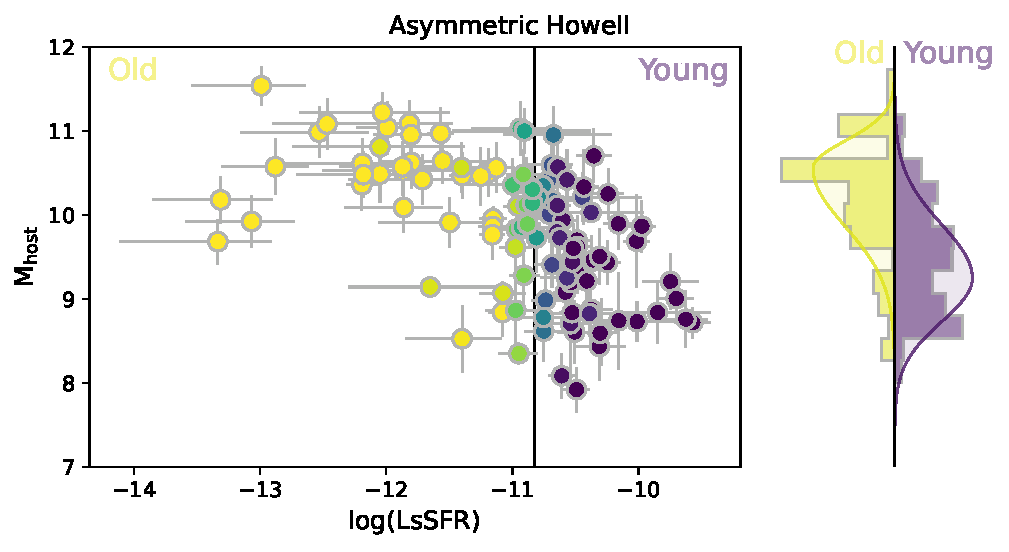
\includegraphics[width=\linewidth]{model_mass_2G2M4S_hist_SED-nonan.pdf}
    \caption{\textit{Main}: SED-fitted host mass ($M_\mathrm{host}$) as a
        function of the LsSFR for SNfactory SNe. The color corresponds to the
        probability, $p_y$, for the SNe~Ia to be young, i.e., to have
        $\log\mathrm{LsSFR} \geq -10.82$ \citep[see][]{rigault2020}.
    \textit{Right}: $p_y$-weighted histogram of the SN masses, as well as the
adjusted model; contributions of the younger and older population are shown in
purple and yellow, respectively.}
    \label{fig:massmodel}
\end{figure}

\begin{table*}
    \centering
    \caption{Comparison of the relative ability of each model to describe the
        data. For each considered model, we report whether the model is
        drifting, its number of free parameters, $-2\ln(L)$ (see
        Eq.~\ref{eq:likelihood}), the AIC and the AIC difference ($\Delta$AIC)
        between this model and the base model used as reference because it has
    the lowest AIC.}
    \label{tab:modelcomp}
    \begin{tabular}{lcccccccc}
        %\hline\hline & & & & & & \\[-0.6em]
        \toprule
        & & & \multicolumn{3}{c}{Fiducial sample (569 SNe)}
            & \multicolumn{3}{c}{Conservative sample (422 SNe)} \\
        \cmidrule(lr){4-6}\cmidrule(lr){7-9}
        Name & drift & $k$ &
        $-2\ln(L)$ & AIC & $\Delta$AIC & $-2\ln(L)$ & AIC & $\Delta$AIC\\[0.2em]
        %\hline & & & & & & \\[-0.6em]
        \midrule

        Asym Howell & $\delta(z)$ & 6
        & 1538.7 & 1550.7 & -- 
        & 1197.4 & 1209.4 & -- \\

        Howell & $\delta(z)$ & 4
        & 1546.6 & 1554.6 & $-4.0$
        & 1205.0 & 1213.0 & $-3.6$ 
        \\

        Asym+Howell & $\delta(z)$ & 5
        & 1546.5 & 1556.5 & $-5.8$
        & 1204.8 & 1214.8 & $-5.4$ 
        \\

        Asymmetric & -- & 3
        & 1593.1 & 1599.1 & $-48.5$
        & 1248.6 & 1254.6 & $-45.2$ 
        \\

        Gaussian & -- & 2
        & 1608.3 & 1612.3 & $-61.6$
        & 1258.2 & 1262.2 & $-52.8$ 
        \\
        \bottomrule
    \end{tabular}
\end{table*}

\begin{table*}
    \centering
    \caption{Best-fit values of the parameters for the mass distribution
    model when applied to the SNfactory dataset only (114 SNe~Ia).}
    \label{tab:modelresults}
    \begin{tabular}{lcccccc}
        %\hline\hline & & & & & & \\[-0.6em]
        \toprule
        Sample  & $\mu_\mathrm{y} $ &
                $\sigma_{-,\mathrm{y}}$ & $\sigma_{+,\mathrm{y}}$
                & $\mu_\mathrm{o} $ &
                $\sigma_{-,\mathrm{o}}$ & $\sigma_{+,\mathrm{o}}$ \\[0.2em]
        %\hline & & & & & & \\[-0.4em]
        \midrule
        SNFactory     & $ 9.34 \pm 0.10 $
                      & $0.51 \pm 0.07 $ & $0.95 \pm 0.07 $
                      & $10.74 \pm 0.48 $
                      & $ 0.48 \pm 0.06 $ & $0.39 \pm 0.06 $ \\
        Fiducial      & $ 9.34 \pm 0.10 $
                      & $0.51 \pm 0.07 $ & $0.95 \pm 0.07 $
                      & $10.74 \pm 0.48 $
                      & $ 0.48 \pm 0.06 $ & $0.39 \pm 0.06 $ \\
        Conservative  & $ 9.23 \pm 0.10 $
                      & $0.47 \pm 0.07 $ & $0.96 \pm 0.07 $
                      & $10.61 \pm 0.48 $
                      & $ 0.41 \pm 0.06 $ & $0.44 \pm 0.06 $ \\
        \bottomrule
    \end{tabular}
\end{table*}

\subsection{Input generation}\label{ssec:inpgen}

Having the two modelings for mass and stretch allows us to pick a redshift and
generate a mass and a stretch value. This will in turn give us the ability to
match the HOSTLIB's masses and replace the stretch values by our \textbf{N21}
modeling's predictions. This is done with the \textit{SNprop} Python
module\footnote{https://github.com/MickaelRigault/snprop}. Given a redshift or
lists of redshift, it takes the expected fraction of young stars using
$\delta(z)$ from Eq.~\ref{eq:delta} then sets a ``young'' or ``old'' flag by
picking a random value $r$ between 0 and 1 and comparing it to said fraction. If
$r < \delta(z)$, then the simulated SN will be young and conversely. The higher
the $z$, the higher the $\delta(z)$, and thus the higher the probability to flag
it young. A graphical explanation is given Fig.~\ref{fig:deltaz}. Stretch and
mass values are then generated with the previous modelings depending whether the
progenitor is considered young or old.

\begin{figure}[]
    \centering
    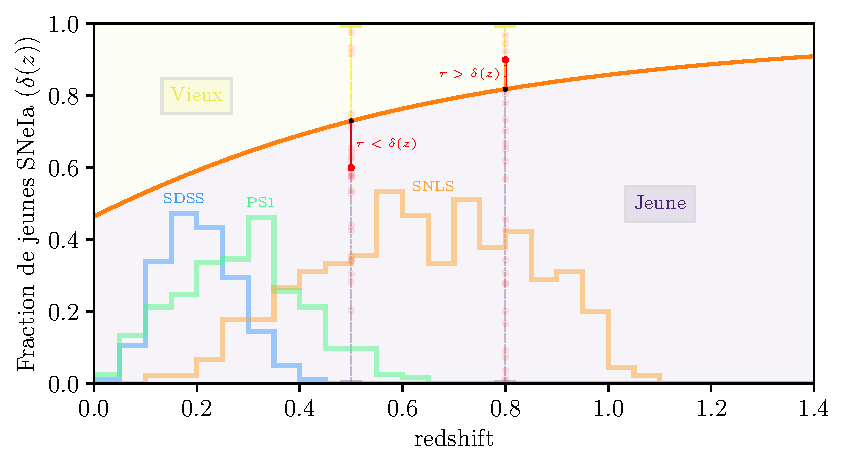
\includegraphics[width=\linewidth]{deltaz_hist_yo-random.pdf}
    \caption{\textit{Orange}: Estimated fraction of young SNe as a function of
        redshift. \textit{Histograms}: Number of SNe in bins of redshift for the
        3 main surveys of the Pantheon sample, not scaled. \textit{Red vertical
        lines}: For each $z$, a random number $a$ between 0 and 1 is picked: if
    it's lower (higher) than $\delta(z)$ at that redshift then the SN will be
young (old), and the distributions of mass and stretch to pick from will follow
this flag.}
    \label{fig:deltaz}
\end{figure}

Diagnostics

\section{Implémentation}\label{sec:snaimpl} 
In order to see the impact of our modeling in the inferred $w$ value, we first
needed to get on-par with the current best work on that matter, working closely
with the SNANA team to recreate the results of \textbf{P21} before using our
HOSTLIB.

\subsection{Description of the tests}\label{ssec:kinds}
We defined 4 ways to simulate SNe depending on the assumptions that can be made.
First, ``SK'' based on \textbf{SK16} where there are no link between a SN and
its host galaxy (in practice using a HOSTLIB without taking the additionnal
correlations into account). Then, ``BP'' based on \textbf{P21} where the $x_1$
and $c$ parameters of the HOSTLIB are generated by asymmetric Gaussian modelings
adjusted to reproduce the observed distributions in nature. The first new
HOSTLIB, dubbed ``NN'', is based on BP but replacing the $x_1$ values following
the previously described procedure, effectively adding one of the consequences
of supposing age as the leading factor between SNe and their environment. The
second new HOSTLIB is dubbed ``NR'', but adds an age column defined by
$\mathrm{age} = \left\{
    \begin{array}{l}
        0 \quad \mathrm{if} \quad r < \delta(z)\\
        1 \quad \mathrm{if} \quad r > \delta(z)
    \end{array}
\right.$ as discussed in Section~\ref{ssec:inpgen}, and an step column in which
we associate a step of $\pm0.065\,\mathrm{mag}$ for young and old SNe
respectively. This step value stems from the other implication of age as the
driving phenomenon under the SNe~Ia correlations, defined in \textbf{R21? B21?}.

In order to replicate the actual datasets on which our stretch model was based
on, i.e. the Pantheon dataset \NN{what do we do of LOWZ?}, we implemented two
approaches of simulation:

\begin{enumerate}
    \item using one DATA sample with (FIND NUMBER) SNe and a unique huge BIASCOR
        sample of (FIND NUMBER), simulations stamped ``FULL'' hereafter;
    \item and a collection of 500 already sample-sized DATA samples that are
        each corrected with the same BIASCOR sample.
\end{enumerate} 

For each of them, finding the scaling factor of NGEN (describe) for each survey
proved crucial to the study. They were computed to have approximately the same
ratio of DATA between surveys at the end of the fitting stage than in Pantheon,
that is shown Table~\ref{tab:ratio}.

LOWZ needed to anchor HD

\begin{table}
    \centering
    \caption{Number of data in Pantheon and relative ratio with respect to the
    smallest sample, LOWZ}
    \label{tab:ratio}
    \begin{tabular}{lcc}
        \toprule
        Survey & Number & Ratio/LOWZ \\
        \midrule
        LOWZ   & 172    & 1.00 \\
        SDSS   & 335    & 1.95 \\
        PS1    & 279    & 1.62 \\
        SNLS   & 236    & 1.37 \\
        \bottomrule
    \end{tabular}
\end{table}

\NN{Melting pot of things to talk about, maybe some in appendix:
\begin{itemize}
    \item Different HOSTLIBs depending on the survey (lowz, highz);
    \item Plot HOSTLIBs parameters
    \item Weigthmaps, plot them
    \item Talk about NGENs and how they are made to fit to the ratio in Pantheon
        \begin{itemize}
            \item Check differences between NN/NR and SK/BP
            \item It might be that having to up the NGENs of non-LOWZ surveys in
                NN/NR wrt SK/BP while keeping LOWZ's NGEN to 20.0 could be a
                result about the impact of this modeling on the generated number
                of low redshift SNe
        \end{itemize}
    \item Inputs:
        \begin{itemize}
            \item $H_0 = \SI{70.0}{km.s^{-1}.Mpc^{-1}}$
            \item $\alpha = 0.145$;
            \item $\beta = 3.1$;
            \item $w = -1$;
            \item $\Omega_m = 0.315$;
            \item $\Omega_\Lambda = 0.685$
        \end{itemize}
    \item Spectroscopic efficiencies
    \item In inputs:
        \begin{itemize}
            \item GENMODEL: SALT2.JLA-B14 for all but LOWZ: SALT2.WFIRST-H17
            \item Intrinsic scatter: G10
            \item SNR > 4 or 2
            \item CUTWIN\_NEPOCH = 5 -5
            \item GENFILTERS? GENRANGE\_REDSHIFT?
            \item GENMEAN, RANGE, SIGMA for x1, c, alpha beta?
        \end{itemize}
    \item For LCFIT stage, SNRMAX = 5 for LOWZ, not the others, beware
        cosmological parameters in that stage
    \item Role of biascor samples
    \item Flavors of biascor samples:
        \begin{itemize}
            \item 1D
            \item 5D
            \item 7D
        \end{itemize}
\end{itemize}}

\subsection{Comparing tests on simulations}
Before comparing the $w$ v $\Omega_m$ values, we looked at the correspondence
between simulated data and actual data to ensure the improvement of our
LsSFR-based approach. The main idea being the evolution of the underlying stretch
distribution as a function of redshift, we represented $x_1$ v $z$ in log-scale
using a 2D hexagonal colored histogram for the simulated data and dots for the
Pantheon values. We also looked at the $x_1$ v $M\mathrm{host}$ plot to ponder
the relationship these two main characteristics of the SNe~Ia on one hand and the
host galaxies on the other (see \ref{fig:P21vN21}). We then computed a 2D kernel
of each set of parameters based on the simulations and determined the associated
$\chi^2$ between the data and the kernels. The results are summarized in Table
\ref{tab:chi2comp} and the code in the \textit{SNprop} module.

\begin{figure*}
    \centering
    
\includegraphics[width=\linewidth]{blank}
    \caption{\textit{Top}: 2D hexagonal histograms of the simulated data using
    the P21 setup in color (left: $x_1$ v $z$, right: $x_1$ v $M_\mathrm{host}$)
    and actual Pantheon data in blue points. \textit{Bottom}: same data but
    2D hexagonal histograms of the simulated program using the N21 improved
    HOSTLIB.}
    \label{fig:P21vN21}
\end{figure*}

\begin{table}
    \centering
    \caption{Comparison of the relative ability of each HOSTLIB implementation
    to describe the data. For each HOSTLIB a 2D KDE is computed from the simulated
    data and used to determine said $\chi^2$.}
    \label{tab:chi2comp}
    \begin{tabular}{c|cc}
        \hline\hline
                & \multicolumn{2}{c}{$\chi^2$}
        \\
        HOSTLIB & $x_1$ v $z$ & $x_1$ v $M_\mathrm{host}$
        \\\hline
        P21     & ????        & ????
        \\
        N21     & ????        & ????
        \\
        \hline
    \end{tabular}
\end{table}

The numerical values follow what was already clear on the figures: it fits best.

\section{Résultats}\label{sec:simres}
What we want is not so much $w$ than $\Delta w$ wrt. best current work. We find
x\% and here are the contours.

\section{Discussion}\label{sec:simdisc}
We expected to have a higher/lower, and we got that.

\section{Conclusion}\label{sec:simccl}

Should be nice.


\clearpage

\thispagestyle{plain}
% \vspace*{-3cm}
\vfill
\minilof
\vfill
\minilot
\vfill

% \bibliographystyle{../main/aa_url}
% \shorthandoff{:}
% \bibliography{../chapters/99_references}

\end{document}
